\section{Quiz}

This remainder of this homework is a series of multiple choice questions related to the word2vec algorithm.

{\bf How to submit:}  Even though these are not coding questions, you will submit your response to
each question in the |src-quiz/submission.py| file.  This file will act as
your 'bubble sheet' for multiple choice questions in this course.  A sample response
might look like this:

\begin{center}
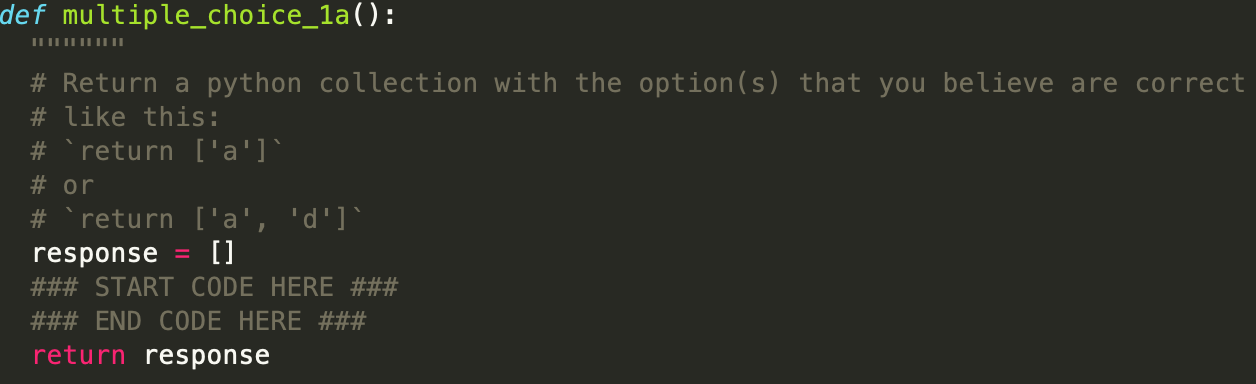
\includegraphics[width=1\textwidth]{sample_question_empty.png}
\end{center}

If you believe that |a| and |b| are the correct responses to this question, you
will type |response = [`a', `b']| between the indicated lines like this:

\begin{center}
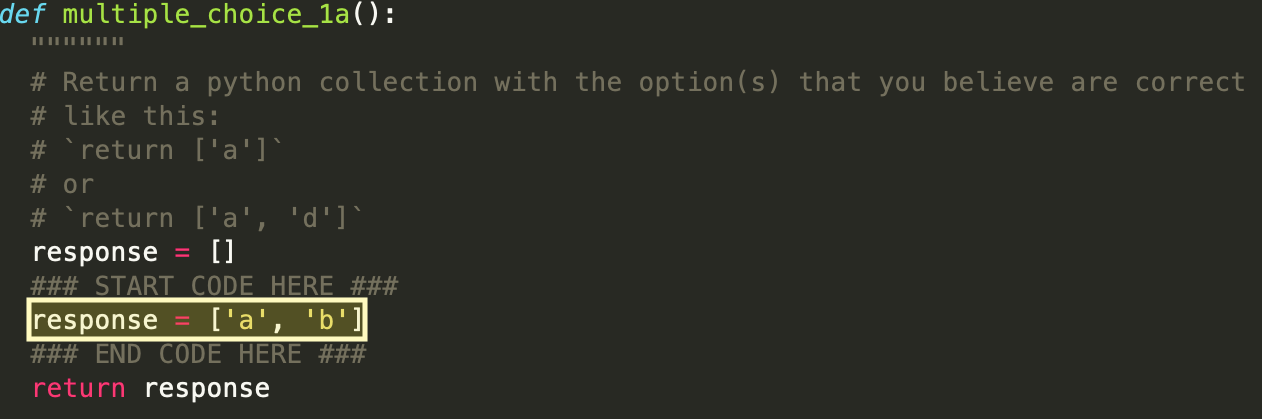
\includegraphics[width=1\textwidth]{sample_question_complete.png}
\end{center}

{\bf How to verify your submission:}
You can run the student version of the autograder locally like all coding
problem sets.  In the case of this problem set, the helper tests will verify
that your responses are within the set of possible choices for each question
(e.g. the helper functions will flag if you forget to answer a question of if
you respond with |[`a', `d']| when the choices are |[`a', `b', `c']|.)  See the
front pages of this assignment for instructions to run the autograder.
\clearpage

{\em {\bf Note:} To answer Questions 1 and 2, review and refer to the Section \ref{sec:char_enc} in this pdf handout.}

\begin{enumerate}[1.]

\item \points{quiz1}

In Assignment 4 we used 256-dimensional word embeddings ($e_\text{word} = 256$). In the Assignment 5 handout you will see that a character embedding size of 50 suffices ($e_\text{char} = 50$).

Select all of the options that explain why the embedding size used for character-level embeddings is typically lower than that used for word embeddings:

\begin{enumerate}[(a)]
\item Words have richer semantic meaning than characters, thus they need higher dimensions to be represented.
\item There are far fewer unique characters than unique words, thus fewer character relationships to represent and fewer features required to capture the difference in meaning between characters.
\item Having a large embedding size of character-level embedding will result in an underfit model.
\end{enumerate}

% ### START CODE HERE ###
% ### END CODE HERE ###

\item Compute the total number of parameters in the character-based embedding model presented below (first image), then do the same for the word-based lookup embedding model (second image), given that in our code, $k = 5$, $V_\text{text}  = 50000$, $V_\text{char} = 96$, $e_\text{word} = 256$ and $e_\text{char} = 50$:

\begin{center}
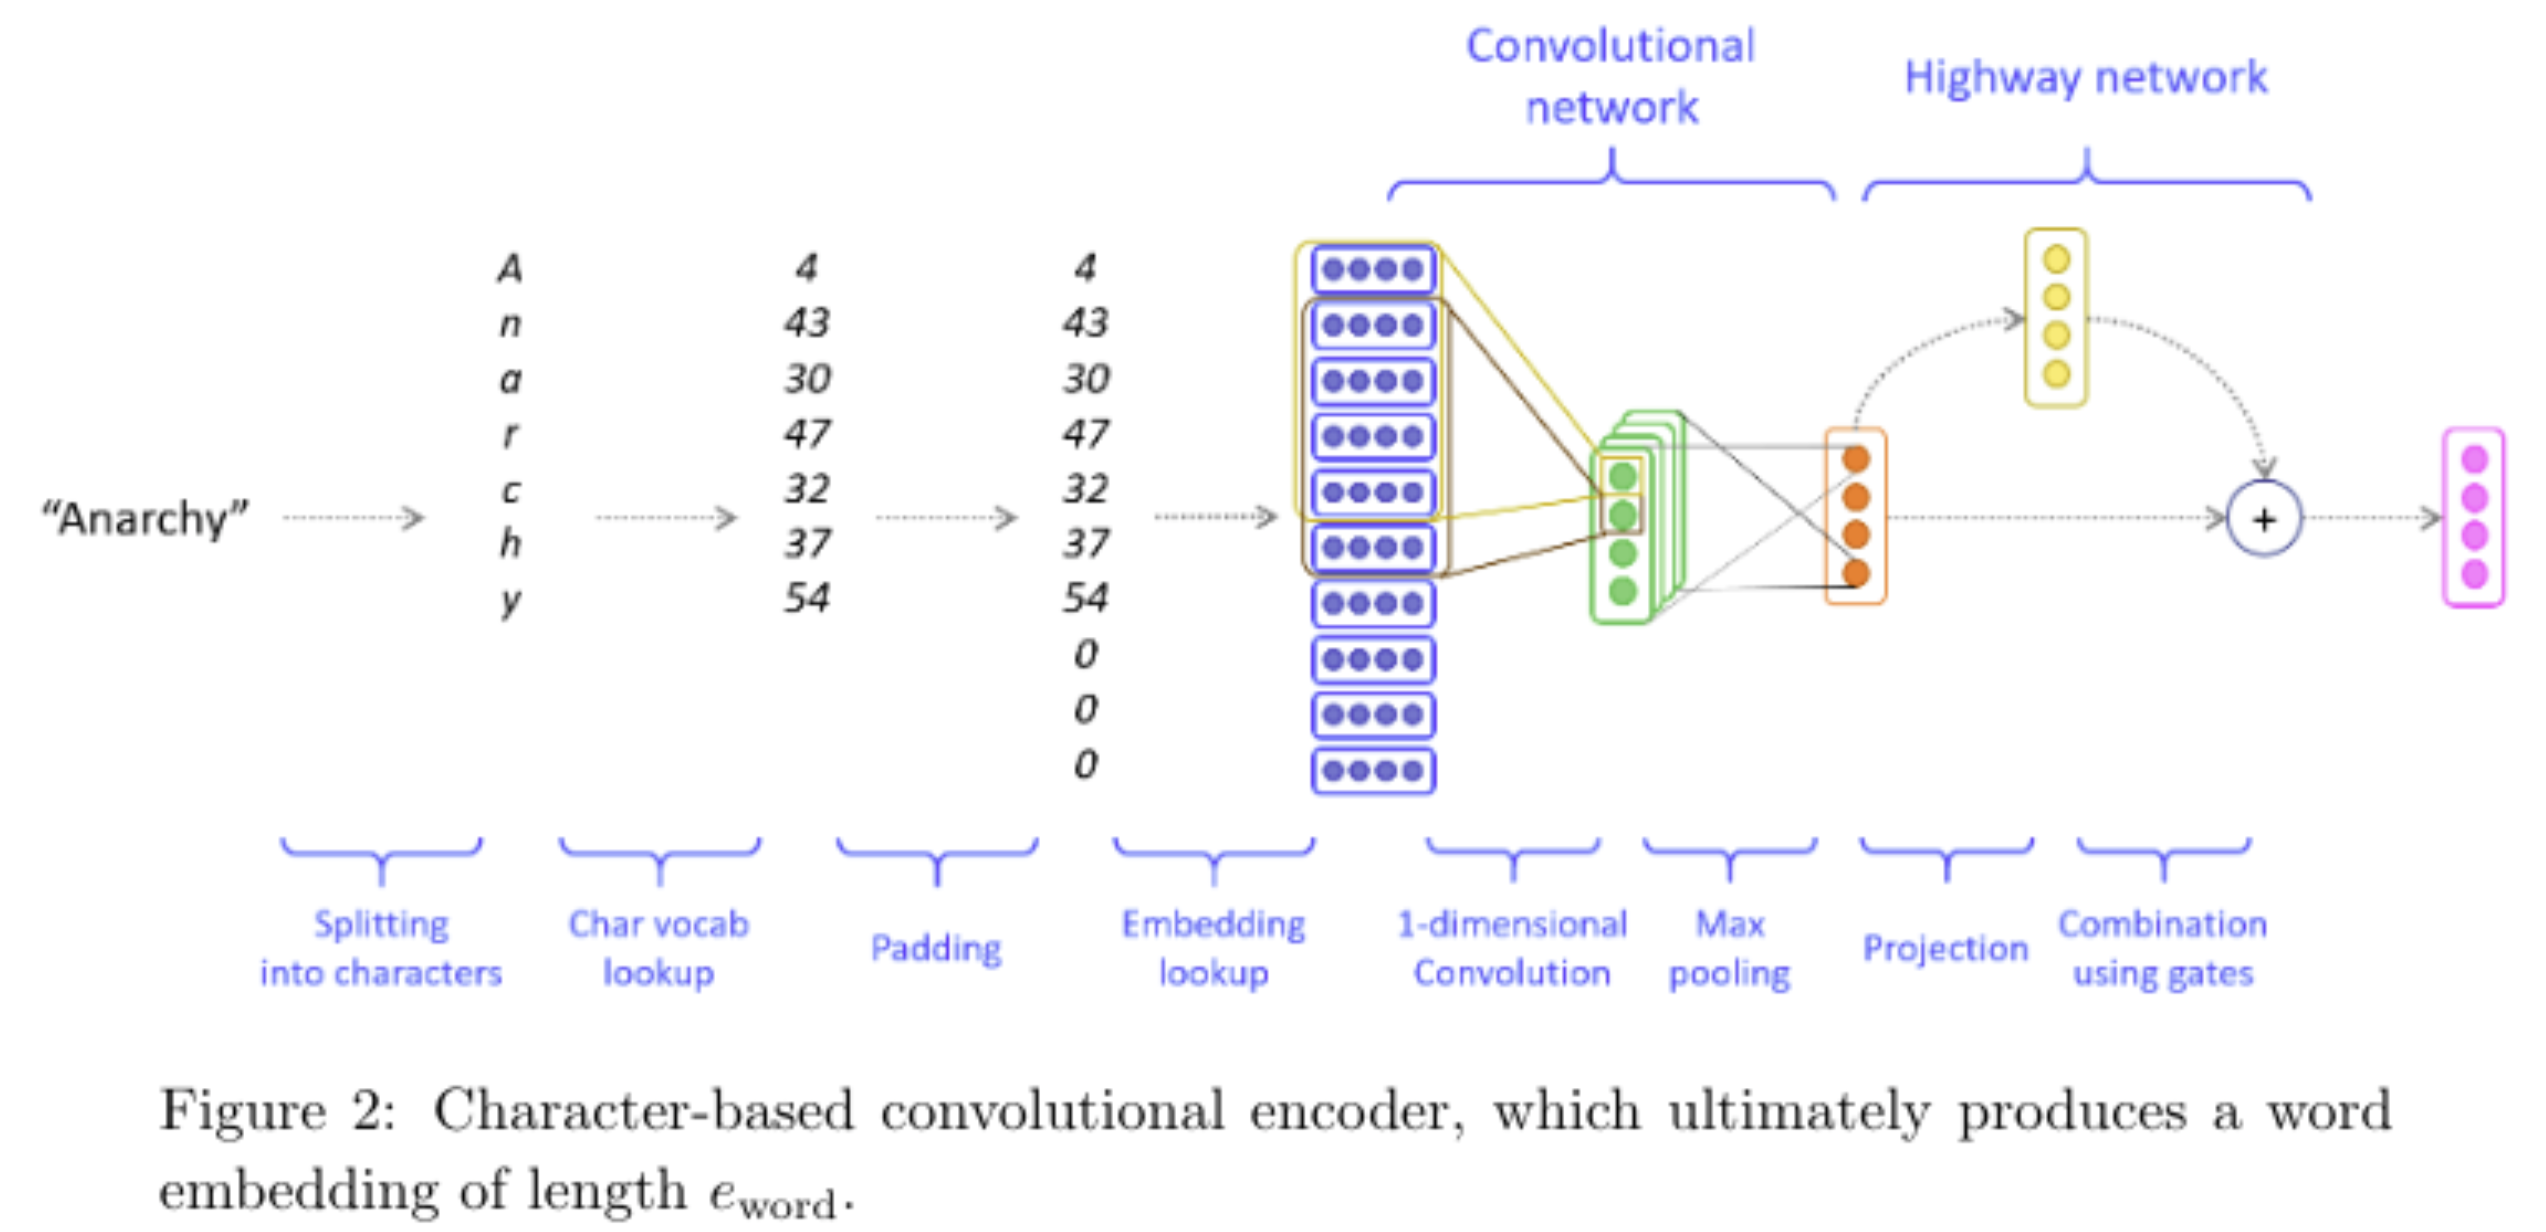
\includegraphics[width=0.75\textwidth]{pre2-1.png}
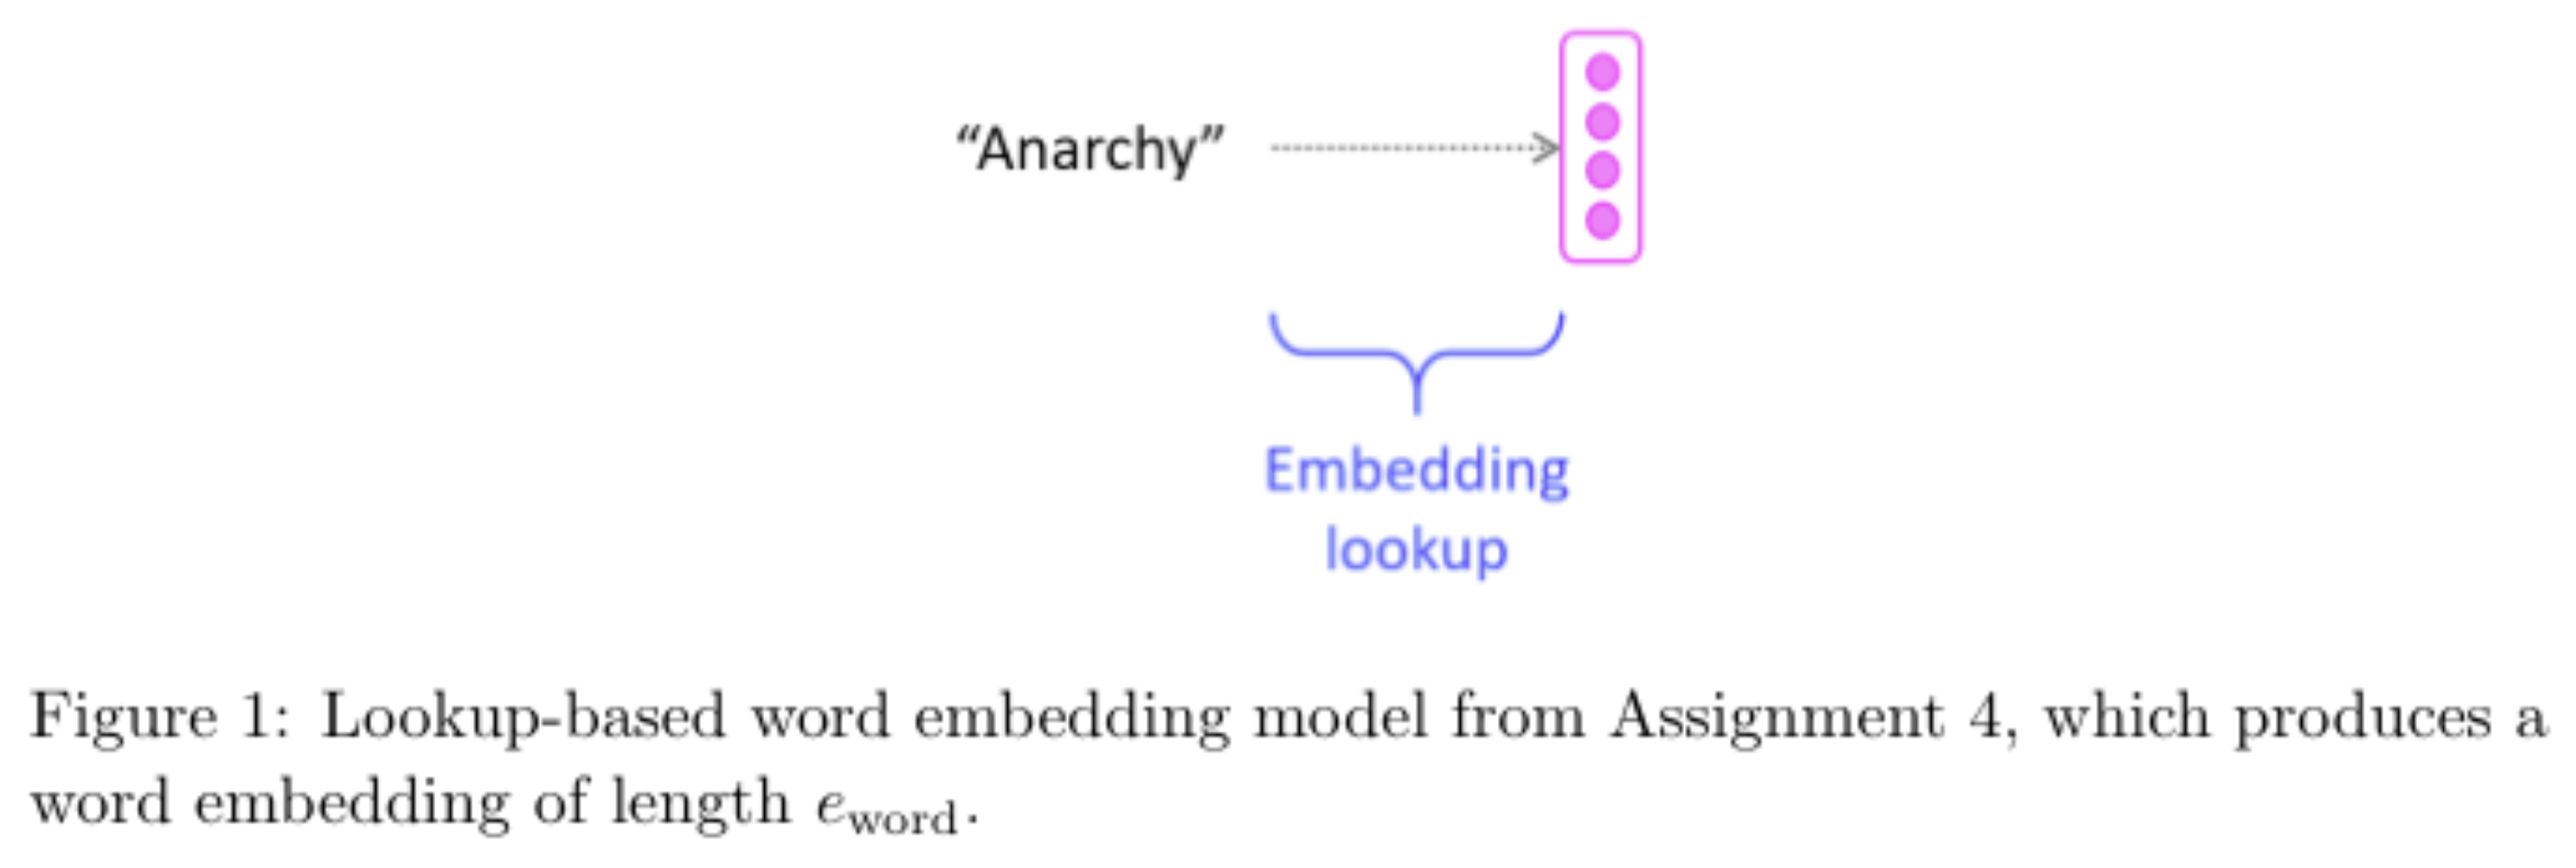
\includegraphics[width=0.75\textwidth]{pre2-2.png}
\end{center}

\begin{enumerate}[2a.]
\item \points{quiz2a}

Total parameter for character-based embedding model

\begin{enumerate}[(a)]
\item $n_\text{paramschar} = 200640$
\item $n_\text{paramschar} = 12800000$
\item $n_\text{paramschar} = 134336$
\end{enumerate}

% ### START CODE HERE ###
% ### END CODE HERE ###

\item \points{quiz2b}

Total parameter for word-based lookup embedding model

\begin{enumerate}[(a)]
\item $n_\text{paramschar} = 200640$
\item $n_\text{paramschar} = 12800000$
\item $n_\text{paramschar} = 134336$
\end{enumerate}

% ### START CODE HERE ###
% ### END CODE HERE ###
\end{enumerate}

\item \points{quiz3}

In lectures, we learned about both max-pooling and average-pooling. Choose all the options that are true regarding pooling (either max or average) operation:

\begin{enumerate}[(a)]
\item {\bf Max pooling} is able to pick up on sparse signals and retain their information, even over large window sizes. By contrast, in average pooling, information from sparse signals is diluted or lost, especially over large window sizes.
\item {\bf Max pooling} is computationally quicker because the gradient only flows through the indices where max occurs, whereas in average pooling gradient flows through all indices.
\item {\bf Average pooling} is good at representing the overall strength of a feature in the input -- by contrast, max pooling is good at being a detector for whether a feature appears somewhere in the input.
\item {\bf Max pooling} reduces the effect of extremes and outliers -- by contrast, these are highlighted by average pooling.
\end{enumerate}

% ### START CODE HERE ###
% ### END CODE HERE ###

\item \points{quiz4}

\begin{center}
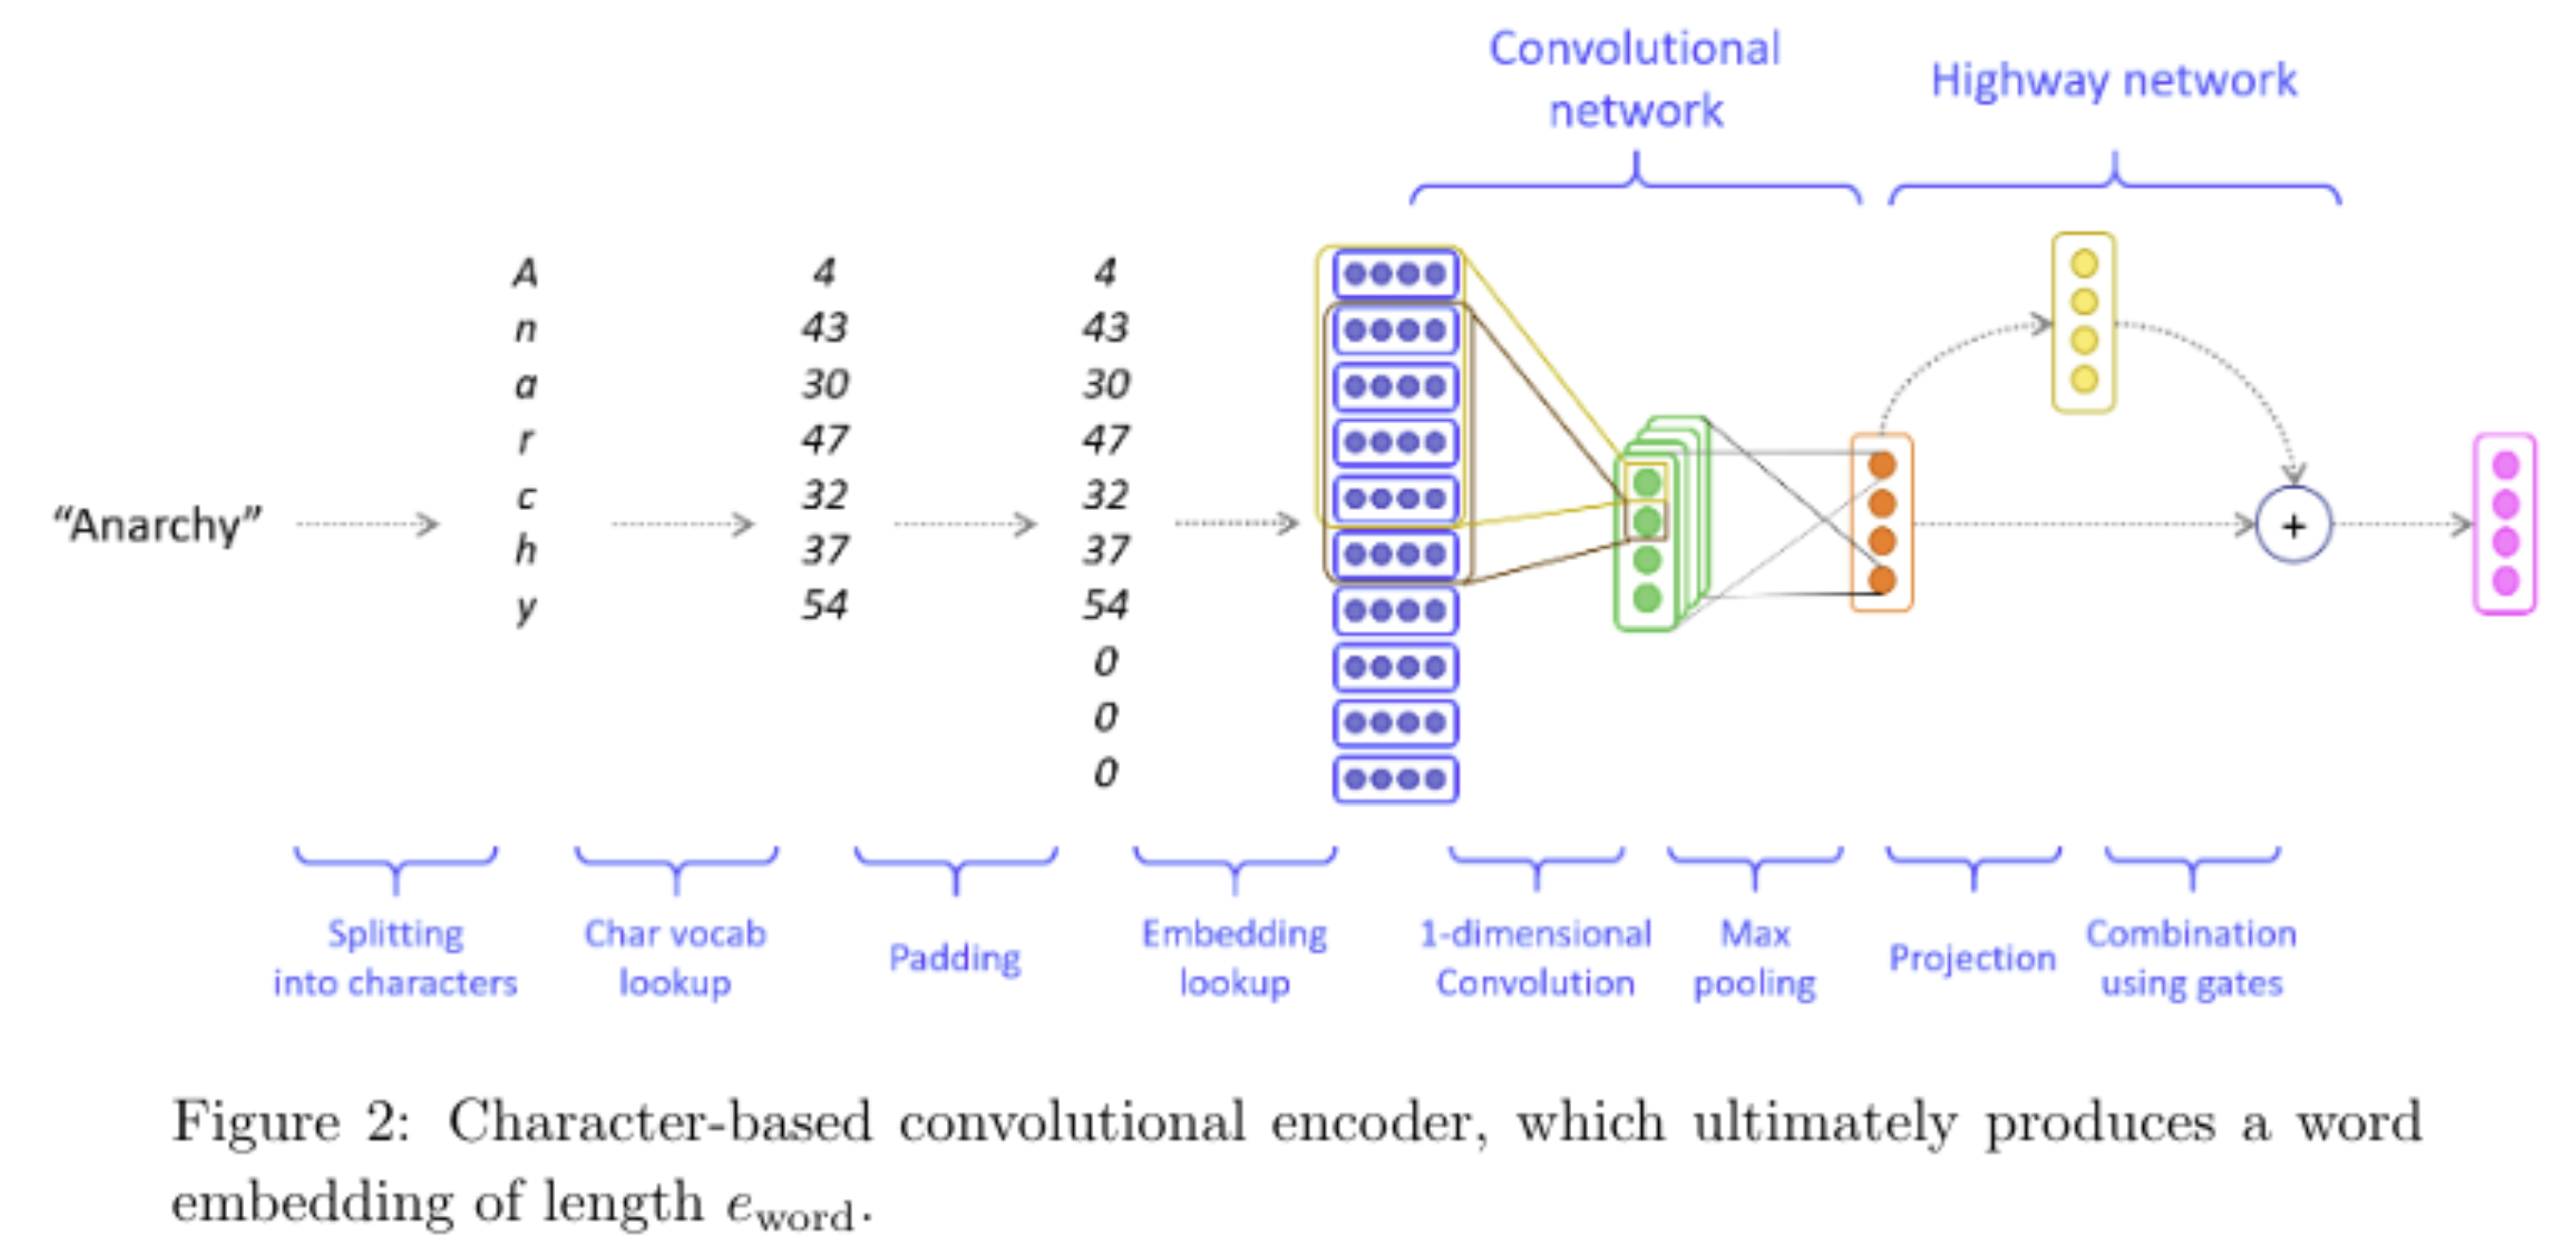
\includegraphics[width=0.75\textwidth]{4-1.png}
\end{center}

In the character-based embedding model, instead of using a 1D convnet we could have used an RNN instead (e.g. feed the sequence of characters into a bidirectional LSTM and combine the hidden states using max-pooling). Choose all the options that explain how char-level CNNs and char-level RNNs differ from each other:

\begin{enumerate}[(a)]
\item The features computed by the CNNs are position-invariant -- for example if the input word is `couscous', and the kernel size is 4, a feature that's computed over the first `cous' is the same as the same feature that's computed over the second `cous'. By contrast, an RNN would have a different hidden state at the end of the first `cous' and at the end of the second `cous'.
\item When a 1D convnet computes features for a given window of the input, those features depend on the window only -- not any other inputs to the left or right. By contrast, an RNN needs to compute the hidden states sequentially, from left to right (and also right to left, if the RNN is bidirectional). Therefore, unlike a RNN, a convnet's features can be computed in parallel, which means that convnets are generally faster, especially for long sequences.
\item Unlike CNNs with long window size, RNNs don't suffer from the vanishing gradient problem and, therefore, can better model the dependency between distant characters in the sequence.w
\end{enumerate}

% ### START CODE HERE ###
% ### END CODE HERE ###

\end{enumerate}
